\subsection{Comparación de estrategias binarias: BS y BSII}

Para la comparación de los resultados obtenidos con cada una de las estrategias binarias se registran las métricas de precisión, \textit{recall} y \textit{f1-socre}. Por claridad se indica que en las gráficas siguientes \ref{fig:Precision} a \ref{fig:F1-score} las etiquetas son:
\begin{itemize}
    \item \textbf{BS\_and:} Búsqueda binaria con conjunción.
    \item \textbf{BS\_or:} Búsqueda binaria con disyunción.
    \item \textbf{BS\_II\_and:} Búsqueda binaria con índice invertido con conjunción.
    \item \textbf{BS\_II\_and:} Búsqueda binaria con índice invertido con disyunción.
\end{itemize}

La precisión indica qué porcentaje de los documentos recuperados se consideran relevantes de acuerdo con la etiqueta de la consulta. Como se esperaba los resultados de las estrategias con conjunción (AND) son mejores que los de disyunción (OR). Esto debido a que hay una mayor probabilidad de que si el documento contienen todos los términos de la consulta sea relevante, mientras que si contiene solo uno de ellos, la probabilidad es muchísimo menor. 

\begin{figure}
    \centering
    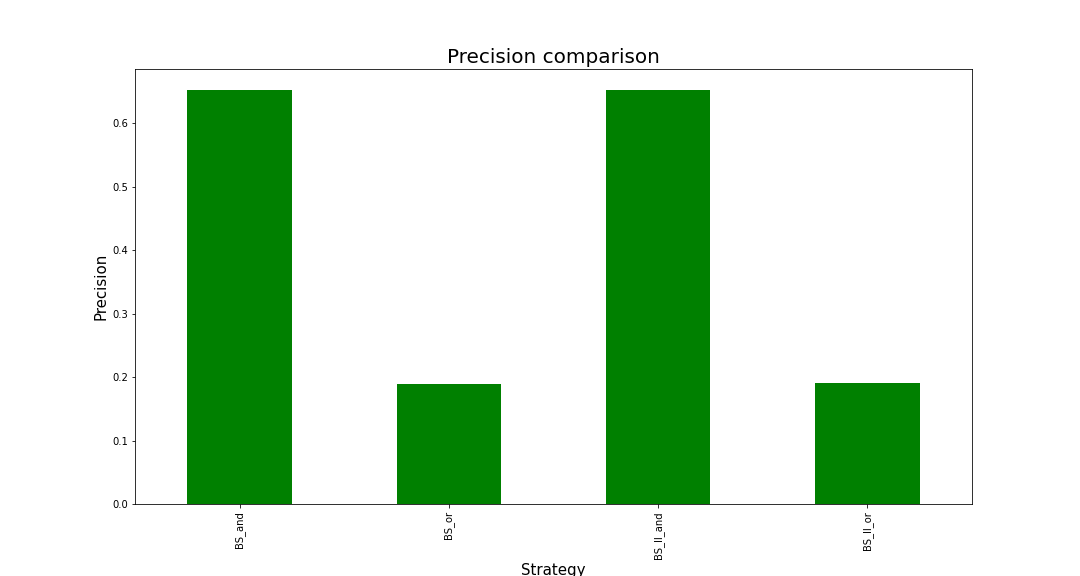
\includegraphics[width=\textwidth]{results/images/BS_precision_comparison.png}
    \caption{Precisión de cada estrategia.}
    \label{fig:Precision}
\end{figure}

El \textit{recall}, por su parte evalúa qué porcentaje de los documentos relevantes fueron recuperados. Con esto en mente, se espera que el resultado de esta métrica con las estrategias de disyunción sea muy buena, mientras que en las estrategias de conjunción resulta mala. 

\begin{figure}
    \centering
    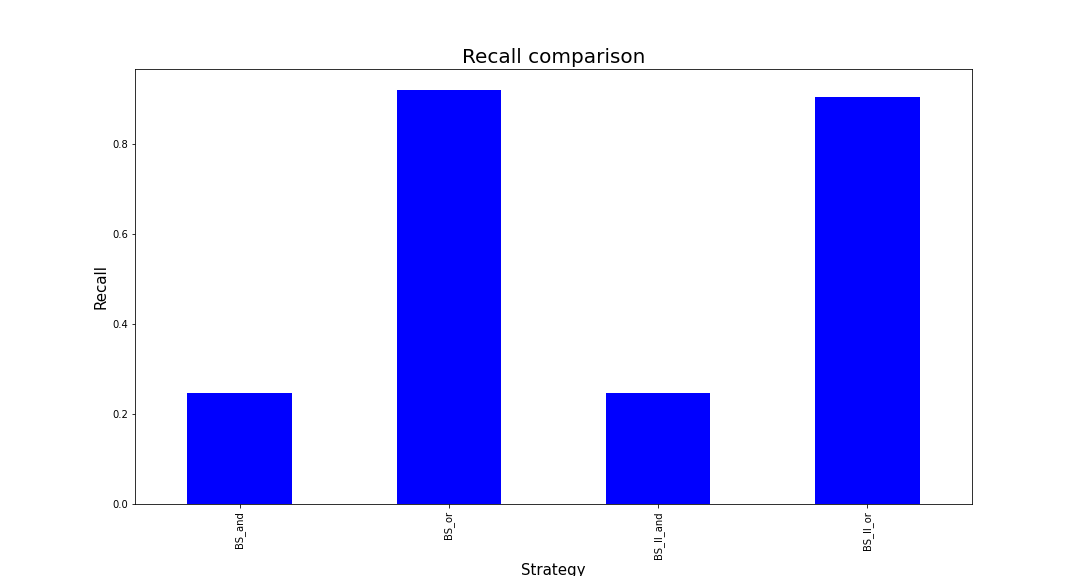
\includegraphics[width=\textwidth]{results/images/BS_recall_comparison.png}
    \caption{\textit{Recall} de cada estrategia.}
    \label{fig:Recall}
\end{figure}

\begin{figure}
    \centering
    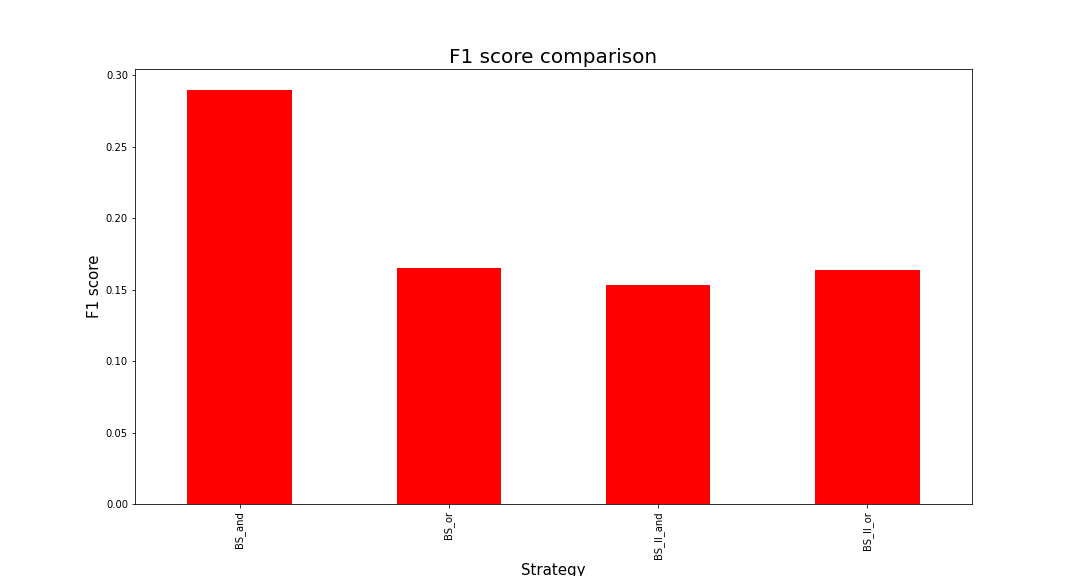
\includegraphics[width=\textwidth]{results/images/BS_f1_comparison.png}
    \caption{F1-score de cada estrategia.}
    \label{fig:F1-score}
\end{figure}


\subsection{Comparación de estrategias clasificadas (\textit{ranked}): RRI, RRDV, GENSIM}

\begin{figure}[H]
    \centering
    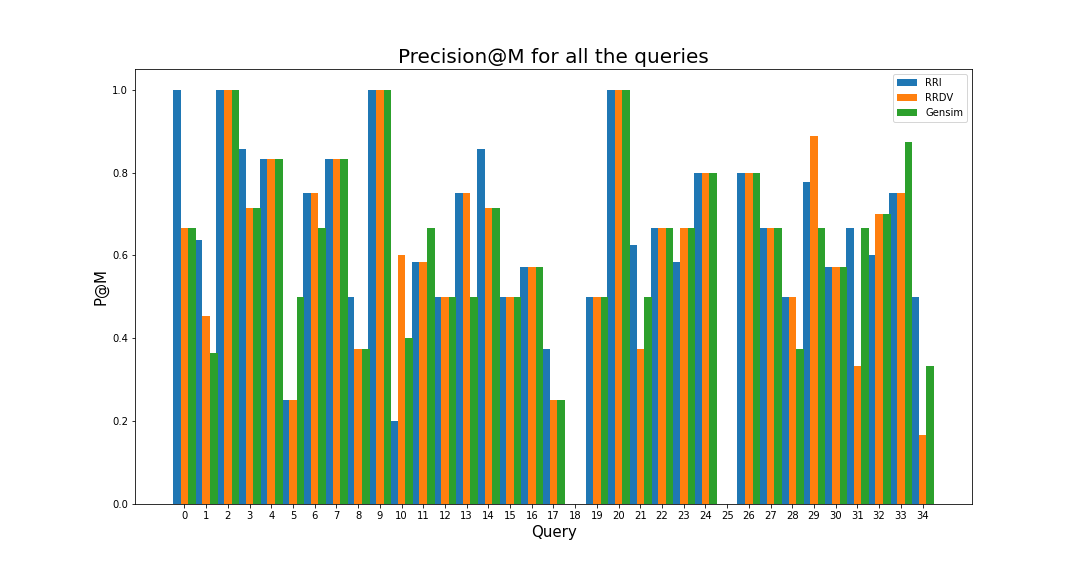
\includegraphics[width=\textwidth]{doc/images/P@M_Ranked.png}
    \caption{Resultados de P@M para todas las queries del data set con las estrategias clasificadas (\textit{ranked})}
    \label{fig:my_label}
\end{figure}

\begin{figure}[H]
    \centering
    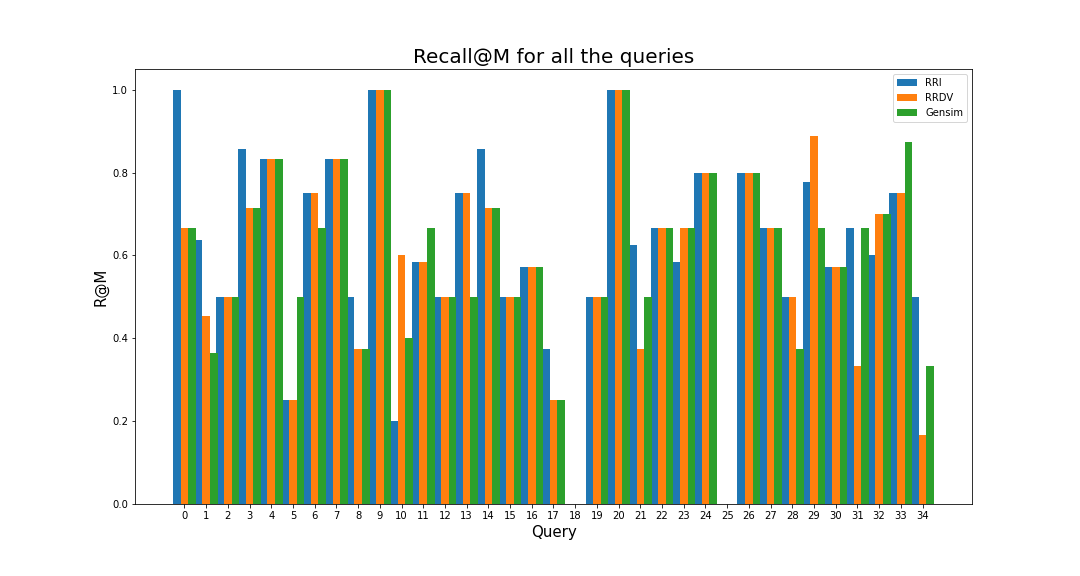
\includegraphics[width=\textwidth]{doc/images/R@M_Ranked.png}
    \caption{Resultados de R@M para todas las queries del data set con las estrategias clasificadas (\textit{ranked})}
    \label{fig:my_label}
\end{figure}


\begin{figure}[H]
    \centering
    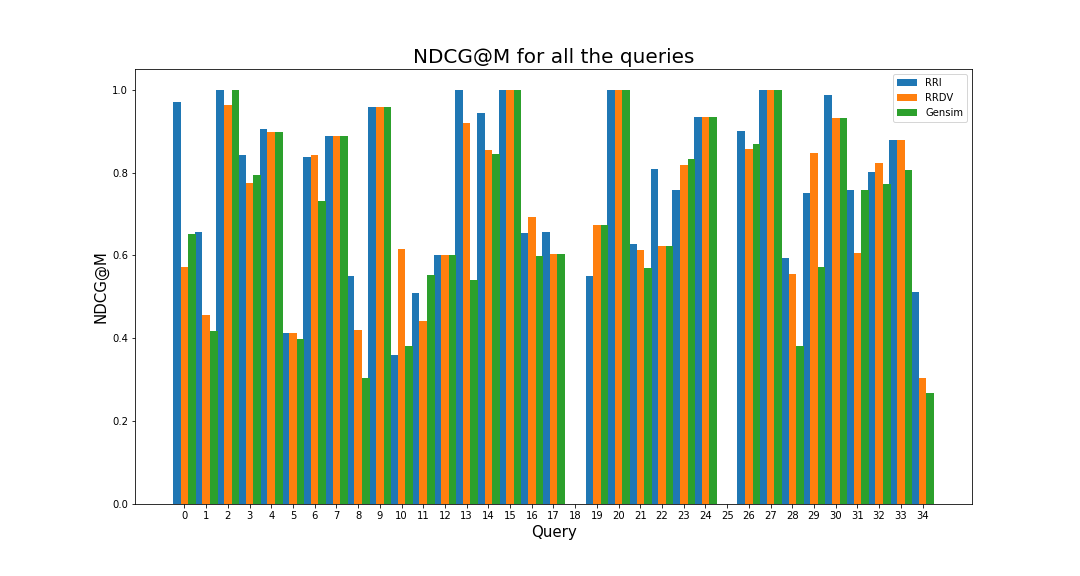
\includegraphics[width=\textwidth]{doc/images/NDCG@M_Ranked.png}
    \caption{Resultados de NDCG@M para todas las queries del data set con las estrategias clasificadas (\textit{ranked})}
    \label{fig:my_label}
\end{figure}


\begin{table}[H]
\centering
\label{tab:rankedResults}
\begin{tabular}{|l|c|c|c|c|}
\hline
\textbf{Estrategia} & \multicolumn{1}{l|}{\textbf{Mean P@M}} & \multicolumn{1}{l|}{\textbf{Mean R@M}} & \multicolumn{1}{l|}{\textbf{Mean NDCG@M}} & \multicolumn{1}{l|}{\textbf{MAP}} \\ \hline
\textbf{RRI} & 0.6287 & 0.6144 & 0.7317 & 0.7340 \\ \hline
\textbf{RRDV} & 0.5923 & 0.5780 & 0.6967 & 0.6972 \\ \hline
\textbf{Gensim} & 0.5955 & 0.5812 & 0.6618 & 0.6592 \\ \hline
\end{tabular}
\caption{Resumen de resultados de desempeño para las estrategias clasificadas (\textit{ranked}).}
\end{table}

